\documentclass[11pt,a4paper]{article}
\usepackage[utf8]{inputenc}
\usepackage[T1]{fontenc}
\usepackage[spanish,es-noshorthands,es-tabla]{babel}

\usepackage[margin=2.3cm]{geometry}
\usepackage{amsmath,amssymb,bm}
\usepackage{booktabs}
\usepackage{graphicx}
\usepackage{float}
\usepackage{caption}
\usepackage[hidelinks]{hyperref}
\usepackage{xcolor}
\usepackage{listings}
\decimalpoint
\captionsetup{font=small,labelfont=bf}
\lstset{basicstyle=\ttfamily\footnotesize,breaklines=true,frame=single}

% Generado por scripts/postprocess.py
\newcommand{\NSims}{63}
\newcommand{\MaxDof}{7{,}8\cdot10^5}
\newcommand{\SGsix}{54{,}5}
\newcommand{\SGone}{106{,}2}
\newcommand{\SGten}{33{,}4}
\newcommand{\PGsix}{40{,}6}
\newcommand{\OpGsix}{5{,}32}
\newcommand{\GtenVsGone}{3{,}2}
\newcommand{\GtenVsGsix}{1{,}6}
\newcommand{\GsixVsGone}{1{,}95}
\newcommand{\RsixRnine}{33}
\newcommand{\RnineArc}{23}
\newcommand{\WinGone}{792}
\newcommand{\WinGten}{616}
\newcommand{\WinGsix}{734}
\newcommand{\WinLossGten}{22}
\newcommand{\WinLossGsix}{7}
\newcommand{\VolGone}{16{,}6}
\newcommand{\VolGten}{17{,}3}
\newcommand{\VolGainGten}{4}
\newcommand{\CaseRatioMin}{7}
\newcommand{\CaseRatioMax}{8}
\newcommand{\ConvLast}{0{,}8}
\newcommand{\ConvOpLast}{0{,}6}
\newcommand{\ConvGoneJump}{34}
\newcommand{\WinklerSi}{37{,}9}
\newcommand{\WinklerKi}{1{,}25}
\newcommand{\WinklerStraight}{29{,}6}
\newcommand{\FemMax}{48{,}0}
\newcommand{\FemPct}{34{,}1}
\newcommand{\FemMaxDev}{27}
\newcommand{\FemPctDev}{-10}
\newcommand{\EratioOpen}{1{,}8617}
\newcommand{\VmOverSone}{0{,}83}
\newcommand{\FuPAHT}{162}
\newcommand{\FuPC}{114}
\newcommand{\FuPLA}{72}
\newcommand{\FuPETG}{62}
\newcommand{\FuABS}{75}
\newcommand{\PAHTvsPLA}{2{,}3}
\newcommand{\PCvsPLA}{1{,}6}
\newcommand{\GainVfiveVseven}{2{,}9}
\newcommand{\GainTotal}{6{,}5}
\newcommand{\FuTenPAHT}{263}
\newcommand{\FuTenPC}{186}
\newcommand{\FuTenPAHTadm}{132}
\newcommand{\FuTenPAHTsost}{79}
\newcommand{\FuFivePLAlo}{25}
\newcommand{\FuFivePLAhi}{50}
\newcommand{\UPLAseven}{0{,}70}
\newcommand{\UPAHTseven}{0{,}31}
\newcommand{\UPCseven}{0{,}44}
\newcommand{\UPETGseven}{0{,}80}
\newcommand{\UPLAten}{0{,}43}
\newcommand{\UPAHTten}{0{,}19}
\newcommand{\OpPAHTseven}{2{,}3}
\newcommand{\OpPLAseven}{3{,}4}
\newcommand{\OpPAHTten}{0{,}9}
\newcommand{\DuctPC}{1{,}3}
\newcommand{\NLoffPLAsix}{161}
\newcommand{\NLrupPLAsix}{201}
\newcommand{\NLoffPAHTsix}{386}
\newcommand{\NLrupPAHTsix}{418}
\newcommand{\NLrupPCsix}{185}
\newcommand{\NLoffPETGsix}{144}
\newcommand{\NLoffPLAten}{295}
\newcommand{\NLoffPAHTten}{703}
\newcommand{\NLrupPAHTten}{800}
\newcommand{\NLrupPCten}{341}
\newcommand{\NLoffPLAone}{79}
\newcommand{\NLyPLAone}{26}
\newcommand{\NLrupPLAone}{90}
\newcommand{\NLratioMin}{2{,}2}
\newcommand{\NLratioMax}{2{,}4}
\newcommand{\NLmeshOff}{3}
\newcommand{\NLmeshRup}{2}
\newcommand{\NLhardOff}{0}
\newcommand{\NLhardRup}{2}
\newcommand{\CrPLAzero}{1{,}0}
\newcommand{\CrPLAten}{3{,}3}
\newcommand{\CrPCzero}{1{,}8}
\newcommand{\CrPCten}{3{,}1}
\newcommand{\CrPAHTzero}{1{,}4}
\newcommand{\CrPAHTten}{3{,}2}
\newcommand{\CrPAHTF}{79}
\newcommand{\CrPLAF}{35}

\newcommand{\sone}{\sigma_1}
\newcommand{\fitbox}[1]{\setbox0\hbox{#1}\ifdim\wd0>\linewidth\resizebox{\linewidth}{!}{\box0}\else\box0\fi}

\title{Selección de material para un gancho en U impreso en 3D\\mediante análisis por elementos finitos}
\author{Cristopher Bustos}
\date{19 de noviembre de 2026}

\begin{document}
\maketitle

\begin{abstract}
\noindent
Se seleccionó el material de impresión de un gancho en U de PLA (barra $\varnothing$12, contorno $57\times60$~mm) que se rompe en servicio en las esquinas. Para ello se desarrolló un modelo de elementos finitos 3D propio, con hexaedros de 8 nodos generados desde vóxeles, integración completa y solución por gradiente conjugado precondicionado. La pieza impresa se representó con un modelo homogeneizado de cáscara y núcleo calibrado con la ley de Gibson--Ashby.

Se resolvieron \NSims{} simulaciones: tres casos de carga, diez geometrías y tres perfiles de impresión, además de estudios de verificación y sensibilidad. El modelo converge (\ConvLast~\% entre las dos mallas más finas, de hasta $\MaxDof$ grados de libertad) y encierra la solución analítica de viga curva de Winkler entre sus dos indicadores de pico.

Se demostró que, con cargas impuestas, el campo de tensiones no depende del módulo de Young, de modo que la capacidad de cada material es proporcional a su resistencia. Con datos de ficha técnica de seis filamentos, el \textbf{PAHT-CF} resulta el material más adecuado: soporta \PAHTvsPLA{} veces la carga del PLA, tiene la mayor HDT (170~°C) y la mayor tenacidad al impacto, y es el más rígido. El PC es la alternativa sin fibra (\PCvsPLA{} veces el PLA), y el PETG queda por debajo del PLA. La geometría es tan determinante como el material: combinada con la geometría óptima (arco con la corona engrosada hacia adentro), la capacidad pasa de \FuFivePLAlo--\FuFivePLAhi{}~N a unos \FuTenPAHT{}~N por pata.

\smallskip\noindent\textbf{Palabras clave:} elementos finitos, vóxeles, hex8, selección de materiales, PLA, PETG, ASA, ABS, PC, PAHT-CF, impresión 3D FDM, viga curva, Gibson--Ashby.
\end{abstract}

\section{Introducción y objetivo}
Un gancho en U de barra $\varnothing$12~mm, impreso por deposición de filamento fundido (FDM), se rompe en servicio en las esquinas. El objetivo de este trabajo es \textbf{seleccionar el material de impresión más adecuado} para la pieza, con un criterio mecánico cuantitativo obtenido de un modelo de elementos finitos (MEF) propio y verificado.

\paragraph{Estado del arte.} El PLA es un poliéster alifático rígido cuyas propiedades dependen de la cristalinidad y del procesamiento~\cite{farah}. En piezas FDM, la orientación de construcción, el espesor de capa y la velocidad de alimentación cambian la resistencia y la rigidez, y las probetas impresas en plano o de canto son las más resistentes~\cite{chacon}. El material impreso es anisótropo~\cite{ahn}, y su resistencia a tracción depende sobre todo de la densidad del relleno, más que de su patrón~\cite{fernandez}. Bajo carga sostenida, la altura de capa y el porcentaje y patrón de relleno controlan la velocidad de fluencia lenta y el tiempo de rotura del PLA~\cite{waseem}. Los ensayos comparativos de fluencia muestran que el tipo de polímero, la temperatura y el nivel de carga son determinantes: el PC es el más estable y el PLA el peor de los polímeros rígidos ensayados~\cite{dogan}. El refuerzo con fibra mejora en general la estabilidad frente a la fluencia~\cite{hausler}.

En cuanto al diseño, una esquina con radio interior nulo produce una singularidad de tensión en elasticidad lineal~\cite{sinclair}, y en barras curvas la fibra interior se carga más que en una viga recta (teoría de Winkler)~\cite{shigley}. Los modelos MEF con hexaedros cúbicos generados directamente desde vóxeles están bien establecidos, incluido el estudio del efecto del tamaño de elemento~\cite{keyak1990,keyak1992}.

\paragraph{Contribuciones.} (i) Una formulación MEF completa y verificada del gancho, con un modelo homogeneizado de la pieza impresa, publicada como código abierto y reproducible (apéndice~\ref{app:codigo}). (ii) La demostración analítica y numérica de que, con cargas impuestas, el campo de tensiones no depende del módulo de Young. (iii) Una comparación cuantitativa de seis materiales con datos de ficha técnica obtenidos con el mismo protocolo de ensayo~\cite{bl-pla,bl-petg,bl-asa,bl-abs,bl-pc,bl-paht}.

\section{Planteamiento del problema}
\subsection{Geometría paramétrica}
El gancho se describe por su eje en el plano de impresión $XY$ y una sección transversal que se barre a lo largo de él. El eje tiene dos patas rectas en $x=\pm a$, desde $y_0$ hasta $y_b$, dos arcos de radio $R_b$ centrados en $(\pm x_c, y_b)$ y un tramo recto superior en $y=y_t$:
\begin{equation}
x_c = a - R_b, \qquad y_b = y_t - R_b, \qquad a = 22{,}5~\text{mm},\; y_0=-30~\text{mm},\; y_t = 24~\text{mm}.
\end{equation}
Para un punto $\mathbf p$ se busca el punto más cercano del eje, de manera analítica en cada tramo. Desde ahí se miden $d_n$, la distancia en el plano positiva hacia afuera de la U, y $z$. El dominio queda definido por una función implícita:
\begin{equation}
\Omega = \{\mathbf p\in\mathbb R^3 : \varphi(\mathbf p)\le 0\},\qquad
\varphi(\mathbf p) = \left(\frac{d_n-\delta(s)}{A(s)}\right)^2 + \left(\frac{z}{B}\right)^2 - 1 .
\end{equation}
$A(s)$ y $B$ son los semiejes de la sección en el plano y en $z$, y $\delta(s)$ desplaza el centro de la sección cuando esta se engrosa. Para las variantes con $\varnothing$12 constante, $A=B=6$~mm y $\delta=0$. En las variantes engrosadas, $A$ pasa de 6~mm a su valor en la corona con una transición suave entre $y=-15$ e $y=5$~mm (medida en el punto del eje), y $\delta = k_\delta(A-6)$, con $k_\delta=-1$ para engrosar hacia adentro manteniendo el contorno exterior.

\begin{table}[htbp]\centering\small
\caption{Variantes de esquina con sección constante.}
\begin{tabular}{lcccc}\toprule
Variante & $R_b$ (eje) & Radio interior $R_b-A$ & Sección & Contorno exterior\\\midrule
v5 (actual, G1) & 6 mm & 0 mm (canto vivo) & $\varnothing$12 & $57\times60$ mm\\
v8 (G4) & 15 mm & 9 mm & $\varnothing$12 & $57\times60$ mm\\
v7 (arco completo, G6) & 22,5 mm & 16,5 mm & $\varnothing$12 & $57\times60$ mm\\\bottomrule
\end{tabular}\end{table}

\subsection{Condición de servicio y casos de carga}
Las puntas de las patas, de 7,5~mm de largo, entran en topes cilíndricos con un agujero de $\varnothing$12,5. La pieza se imprime acostada, así que el plano de la U coincide con el plano de las capas. Se estudiaron tres casos de carga, con una fuerza de referencia de 100~N por pata (200~N en total). El caso~3, la apertura de la U con la fuerza en los extremos de las patas, reproduce la falla observada en las esquinas y es el caso de diseño.

\begin{table}[htbp]\centering\small
\caption{Casos de carga.}
\begin{tabular}{lp{2.8cm}p{3.6cm}p{3.6cm}c}\toprule
Caso & Descripción & Apoyo $\Gamma_u$ & Superficie cargada $\Gamma_t$ & Dirección\\\midrule
1 & Tiro del tramo superior & Patas empotradas en la zona de los topes ($y\le-22{,}5$ mm) & Cara interior del tramo superior, $|x|\le10$ mm & $(0,1,0)$\\
2 & Apertura a media altura & Igual que el caso 1 & Cara exterior de las patas, $-8\le y\le2$ mm & $(\pm1,0,0)$\\
3 (diseño) & Apertura en los extremos & Sección de simetría $x=0$ & Cara exterior de las patas, $y\le-22{,}5$ mm & $(\pm1,0,0)$\\\bottomrule
\end{tabular}\end{table}

\subsection{Variables de decisión}
La variable principal es el material. Las variables secundarias son la geometría de la esquina y el perfil de impresión: 2 paredes con 15~\% de relleno (el actual) o 5 paredes con 25~\% de relleno gyroid (el recomendado).

\section{Modelación matemática}
El gancho se modela como un sólido elástico lineal tridimensional, en régimen cuasiestático y con pequeñas deformaciones, resuelto por el método de Galerkin con elementos hexaédricos trilineales~\cite{zienkiewicz}.

\subsection{Forma fuerte}
Sea $\Omega$ el dominio anterior con frontera $\partial\Omega=\Gamma_u\cup\Gamma_t\cup\Gamma_0$. Se busca $\mathbf u:\Omega\to\mathbb R^3$ tal que
\begin{equation}
\begin{aligned}
&\nabla\cdot\bm\sigma = \mathbf 0 \text{ en } \Omega, &&
\bm\varepsilon = \tfrac12(\nabla\mathbf u+\nabla\mathbf u^T), &&
\bm\sigma = \mathbb C(\mathbf x):\bm\varepsilon,\\
&\mathbf u = \mathbf 0 \text{ en }\Gamma_u, &&
\bm\sigma\mathbf n = \bar{\mathbf t}\text{ en }\Gamma_t, &&
\bm\sigma\mathbf n = \mathbf 0\text{ en }\Gamma_0 .
\end{aligned}
\end{equation}
El peso propio ($\approx0{,}2$~N frente a 200~N) se desprecia. El tensor isótropo es $C_{ijkl}=\lambda\delta_{ij}\delta_{kl}+\mu(\delta_{ik}\delta_{jl}+\delta_{il}\delta_{jk})$, con $\lambda=E\nu/((1+\nu)(1-2\nu))$ y $\mu=E/(2(1+\nu))$; $E(\mathbf x)$ varía según el modelo de cáscara y núcleo y $\nu$ es uniforme.

\subsection{Forma débil}
Sea $V=\{\mathbf v\in[H^1(\Omega)]^3:\mathbf v=\mathbf 0 \text{ en }\Gamma_u\}$. Hallar $\mathbf u\in V$ tal que
\begin{equation}
a(\mathbf u,\mathbf v)=\int_\Omega \bm\varepsilon(\mathbf v):\mathbb C:\bm\varepsilon(\mathbf u)\,d\Omega
= \ell(\mathbf v)=\int_{\Gamma_t}\bar{\mathbf t}\cdot\mathbf v\,d\Gamma\qquad\forall\mathbf v\in V.
\end{equation}
La forma $a$ es bilineal, simétrica, continua y, por la desigualdad de Korn, $V$-elíptica; por Lax--Milgram la solución existe, es única y minimiza la energía potencial total $\Pi(\mathbf v)=\frac12a(\mathbf v,\mathbf v)-\ell(\mathbf v)$.

\subsection{Discretización, elemento y cuadratura}
Una grilla cartesiana de cubos de lado $h$, alineada con los planos coordenados, cubre $\Omega$; un cubo es elemento si su centroide cumple $\varphi(\mathbf x_c)\le0$~\cite{keyak1990,keyak1992}. Las funciones de forma trilineales son $N_a=\frac18(1+\xi\xi_a)(1+\eta\eta_a)(1+\zeta\zeta_a)$. Como todos los elementos son cubos idénticos, $\mathbf J=\frac h2\mathbf I$ y $\nabla_{\mathbf x}N_a=\frac2h\nabla_{\bm\xi}N_a$. Con $\bm\varepsilon=\mathbf B\mathbf u_e$ en notación de Voigt,
\begin{equation}
\mathbf K_e=\sum_{i,j,k=1}^{2}\mathbf B^T(\xi_i,\eta_j,\zeta_k)\,\mathbf D\,\mathbf B(\xi_i,\eta_j,\zeta_k)\det\mathbf J,\qquad \xi_i,\eta_j,\zeta_k=\pm\tfrac1{\sqrt3}.
\end{equation}
La regla $2\times2\times2$ es exacta para el cubo y no introduce modos espurios (el elemento tiene exactamente seis autovalores nulos, verificado en las pruebas automáticas). Como $\mathbf D$ es lineal en $E$, se calcula una sola matriz unitaria y se escala por elemento: $\mathbf K_e=E_e\hat{\mathbf K}(\nu)$.

\subsection{Ensamblaje, cargas y condiciones de borde}
$\mathbf K=\sum_e\mathbf L_e^T\mathbf K_e\mathbf L_e$ se arma en formato COO y se convierte a CSR (a lo más 81 entradas no nulas por fila). La tracción en $\Gamma_t$ se reemplaza por fuerzas nodales iguales $\mathbf f_i=(F/n)\,\mathbf d_i$ sobre los $n$ nodos de superficie de la zona cargada (nodos que pertenecen a menos de 8 elementos). Los grados de libertad impuestos se eliminan por partición, $\mathbf K_{ff}\mathbf U_f=\mathbf F_f$. En el caso~3 las cargas son autoequilibradas y simétricas respecto de $x=0$: fijar los tres componentes en ese plano elimina el movimiento de cuerpo rígido sin introducir reacciones netas, y solo restringe localmente la contracción de Poisson de esa sección.

\subsection{Solución y recuperación de tensiones}
Para menos de $6\cdot10^4$ incógnitas se usa LU dispersa; para el resto, gradiente conjugado precondicionado con Jacobi ($\mathbf M=\operatorname{diag}\mathbf K_{ff}$), con parada en $\|\mathbf r_k\|/\|\mathbf F_f\|\le10^{-9}$ y verificación posterior del residuo real. La tensión se evalúa en el centroide de cada elemento, $\bm\sigma_e=E_e\hat{\mathbf D}(\nu)\mathbf B(\mathbf 0)\mathbf u_e$, y se reportan dos indicadores sobre la cáscara impresa: el máximo de $\sone$ y su percentil 99,8, menos sensible a un vóxel aislado en un canto vivo. El núcleo de relleno se excluye porque su tensión homogeneizada no representa la de los filamentos.

\section{Modelo de material de la pieza impresa}
\subsection{Homogeneización cáscara--núcleo}
Una pieza FDM está formada por una cáscara densa y un núcleo de relleno poroso:
\begin{equation}
E(\mathbf x)=\begin{cases}E_s & d(\mathbf x)\le t_s\\ k\,E_s & d(\mathbf x)>t_s\end{cases},\qquad
d(\mathbf x)\approx\left(1-\sqrt{\varphi(\mathbf x)+1}\right)\min(A,B),
\end{equation}
con $t_s\approx$ número de paredes $\times$ 0,42~mm. El factor $k$ se estima con la ley de Gibson--Ashby~\cite{gibson}, $E^*/E_s=C(\rho^*/\rho_s)^n$, $C\approx1$, $n=1\ldots2$.

\begin{table}[htbp]\centering\small
\caption{Parámetros de los perfiles de impresión.}
\begin{tabular}{lccccc}\toprule
Perfil & $t_s$ & $\rho^*/\rho_s$ & Rango de $k$ & $k$ usado & Sensibilidad\\\midrule
2 paredes, 15 \% & 1,0 mm & 0,15 & 0,0225--0,15 & 0,08 & 0,0225 y 0,15\\
5 paredes, 25 \% gyroid & 2,2 mm & 0,25 & 0,0625--0,25 & 0,25 & 0,0625\\
Macizo & — & 1 & 1 & 1 & —\\\bottomrule
\end{tabular}\end{table}

\subsection{Teorema de escalado: la tensión no depende de $E_s$}
Si $E(\mathbf x)=E_s\,e(\mathbf x)$ con $\nu$ uniforme, entonces $\mathbb C=E_s\hat{\mathbb C}$ y $a=E_s\hat a$. Si $\hat{\mathbf u}$ resuelve $\hat a(\hat{\mathbf u},\mathbf v)=\ell(\mathbf v)$, por unicidad $\mathbf u=\hat{\mathbf u}/E_s$ y
\begin{equation}
\bm\sigma=E_s\hat{\mathbb C}:\bm\varepsilon(\hat{\mathbf u}/E_s)=\hat{\mathbb C}:\bm\varepsilon(\hat{\mathbf u})
\;\Longrightarrow\;\frac{\partial\bm\sigma}{\partial E_s}=\mathbf 0,\qquad \mathbf u\propto\frac1{E_s}.
\end{equation}
Con cargas impuestas, el campo de tensiones de una geometría, caso y perfil es el mismo para todos los materiales. Basta un campo por combinación; el material entra por su resistencia, su rigidez, su ductilidad y tenacidad, y su comportamiento en el tiempo y con la temperatura.

\section{Criterios de falla, capacidad y rigidez}
Se usa el criterio de la tensión principal máxima con la resistencia a tracción en el plano de las capas, $\sigma_{1,\max}\le\sigma_{t,XY}/FS$. En la corona de la v7 el estado es casi uniaxial ($\sigma_{VM}/\sone=\VmOverSone$ en el pico). Por linealidad,
\begin{equation}
F_u=F_{ref}\frac{\sigma_{t,XY}}{\sigma_{1,\max}(F_{ref})},\qquad F_{adm}=\frac{F_u}{FS},\qquad
\Delta=\Delta_{ref}\frac{E_{ref}}{E_{f,XY}}\frac{F}{F_{ref}},
\end{equation}
con $F_{ref}=100$~N por pata y $E_{ref}=3500$~MPa. Para la apertura se usa el módulo de flexión (ISO 178). La reserva de ductilidad se mide como $\varepsilon_b/\varepsilon_{pico}$ con $\varepsilon_{pico}=\sigma_t/E_t$. Para carga permanente se adopta $\sigma_{sost}\le\eta\,\sigma_{t,XY}$ con $\eta=0{,}3$, hipótesis de diseño de este trabajo.

\section{Materiales candidatos}
\begin{table}[htbp]\centering\small
\caption{Propiedades de ficha técnica (probetas 100 \% macizas, recocidas y secas; ISO 527, 178, 179 y 75).}
\begin{tabular}{lrrrrrrrr}\toprule
Material & $E_t$ XY & $E_f$ XY & $\sigma_t$ XY & $\sigma_t$ Z & $\varepsilon_b$ XY & Impacto & HDT & Ref.\\
& [MPa] & [MPa] & [MPa] & [MPa] & [\%] & [kJ/m$^2$] & [°C] & \\\midrule
PLA Basic & 2680 & 2750 & 39 & 35 & 12,2 & 7,9 & 54 & \cite{bl-pla}\\
PETG HF & 1810 & 2050 & 34 & 23 & 8,6 & 6,2 & 62 & \cite{bl-petg}\\
ASA & 2450 & 1920 & 37 & 31 & 9,2 & 19,6 & 92 & \cite{bl-asa}\\
ABS & 3800 & 1880 & 41 & 32 & 10,5 & 21,5 & 84 & \cite{bl-abs}\\
PC & 2110 & 2310 & 62 & 56 & 3,8 & 7,5 & 117 & \cite{bl-pc}\\
PAHT-CF & 3860 & 4120 & 88 & 64 & 10,4 & 22,8 & 170 & \cite{bl-paht}\\\bottomrule
\end{tabular}\end{table}
El PETG HF tiene menor resistencia que el PLA en XY y en Z; su ventaja es solo térmica. El PC tiene la mayor resistencia entre capas de los polímeros sin fibra, pero el menor alargamiento. El PAHT-CF duplica la resistencia del PLA y tiene la mayor HDT, aunque sus propiedades están medidas en seco y absorbe 0,88~\% de agua. Se adoptó $\nu=0{,}35$ para todos (sección~\ref{sec:verif}).

\section{Simulaciones realizadas}
Se resolvieron \NSims{} simulaciones en cuatro series: A (caso 1), B (caso 2), C (caso 3, diez geometrías) y D (verificación y sensibilidad). Todas usan $E_{ref}=3500$~MPa y $\nu=0{,}35$ salvo en los estudios de sensibilidad, y $F=100$~N por pata. La lista completa está en \texttt{ganchofem/series.py} y los resultados en \texttt{results/simulaciones.csv}.
\begin{table}[htbp]
\centering\small
\caption{Tamaño y costo de los modelos (valores registrados por el solver de este repositorio).}
\label{tab:tamanos}
\fitbox{
\begin{tabular}{lrrrrlrrr}
\toprule
Modelo & $h$ [mm] & Elementos & GDL libres & nnz($K_{ff}$) & Solver & Iter. & Residuo & $t$ [s] \\
\midrule
G6 macizo & 1{,}00 & 14\,856 & 55\,140 & 3{,}8$\cdot10^6$ & LU disperso & — & 7{,}3e-11 & 23 \\
G6 macizo & 0{,}75 & 36\,564 & 128\,658 & 9{,}3$\cdot10^6$ & PCG-Jacobi & 608 & 1{,}0e-09 & 64 \\
G6, 5 paredes & 0{,}50 & 120\,460 & 403\,548 & 23{,}8$\cdot10^6$ & PCG-Jacobi & 1048 & 1{,}0e-09 & 154 \\
G1, 2 paredes, $k=0{,}0225$ & 0{,}50 & 132\,660 & 442\,212 & 25{,}9$\cdot10^6$ & PCG-Jacobi & 1688 & 1{,}3e-09 & 366 \\
G10, 5 paredes & 0{,}50 & 138\,620 & 459\,750 & 27{,}2$\cdot10^6$ & PCG-Jacobi & 1032 & 1{,}0e-09 & 204 \\
G6 macizo & 0{,}40 & 237\,032 & 776\,724 & 50{,}6$\cdot10^6$ & PCG-Jacobi & 1140 & 1{,}1e-09 & 284 \\
\bottomrule
\end{tabular}}
\par\smallskip\parbox{0.95\linewidth}{\footnotesize Tiempos en un contenedor de 4 núcleos con 3 simulaciones en paralelo.}
\end{table}


\section{Verificación y sensibilidad}\label{sec:verif}
\begin{table}[htbp]
\centering\small
\caption{Independencia de la tensión respecto de $E$.}
\label{tab:E}
\fitbox{
\begin{tabular}{lrrrr}
\toprule
Corrida (G6, 5 paredes, $h=0{,}5$ mm) & $E$ [MPa] & $\sigma_{1,\max}$ [MPa] & Percentil 99,8 [MPa] & Apertura [mm] \\
\midrule
Referencia & 3500 & 54{,}48 & 40{,}63 & 5{,}3249 \\
Módulo de flexión del ABS & 1880 & 54{,}48 & 40{,}63 & 9{,}9134 \\
\bottomrule
\end{tabular}}
\end{table}

\begin{table}[htbp]
\centering\small
\caption{Sensibilidad al coeficiente de Poisson (G6, 5 paredes).}
\label{tab:nu}
\fitbox{
\begin{tabular}{rrrr}
\toprule
$\nu$ & $\sigma_{1,\max}$ [MPa] & Variación & Apertura [mm] \\
\midrule
0{,}30 & 54{,}08 & -0{,}7 \% & 5{,}352 \\
0{,}35 & 54{,}48 & referencia & 5{,}325 \\
0{,}40 & 54{,}97 & +0{,}9 \% & 5{,}288 \\
\bottomrule
\end{tabular}}
\end{table}

\begin{table}[htbp]
\centering\small
\caption{Sensibilidad al módulo del relleno.}
\label{tab:k}
\fitbox{
\begin{tabular}{llrrr}
\toprule
Geometría y perfil & $k$ & $\sigma_{1,\max}$ [MPa] & Variación & Apertura [mm] \\
\midrule
G6, 5 paredes & 0,25 (adoptado) & 54{,}5 & referencia & 5{,}32 \\
G6, 5 paredes & 0,0625 ($n=2$) & 56{,}7 & +4{,}0 \% & 5{,}76 \\
G1, 2 paredes & 0,15 ($n=1$) & 143{,}5 & -8{,}3 \% & 11{,}07 \\
G1, 2 paredes & 0,08 (adoptado) & 156{,}4 & referencia & 12{,}59 \\
G1, 2 paredes & 0,0225 ($n=2$) & 177{,}9 & +13{,}7 \% & 15{,}91 \\
\bottomrule
\end{tabular}}
\end{table}

\begin{table}[htbp]
\centering\small
\caption{Convergencia de malla (macizo, caso 3; tensiones en MPa).}
\label{tab:conv}
\fitbox{
\begin{tabular}{rrrrr}
\toprule
$h$ [mm] & G6: $\sigma_{1,\max}$ & G6: P99,8 & G6: apertura [mm] & G1: $\sigma_{1,\max}$ \\
\midrule
1{,}00 & 41{,}86 & 34{,}39 & 4{,}656 & 69{,}01 \\
0{,}75 & 45{,}25 & 33{,}56 & 4{,}471 & 67{,}03 \\
0{,}50 & 47{,}58 & 34{,}21 & 4{,}533 & 89{,}87 \\
0{,}40 & 47{,}96 & 34{,}11 & 4{,}507 & — \\
\bottomrule
\end{tabular}}
\end{table}

\paragraph{Independencia de $E$.} La tensión es idéntica y el cociente de aperturas vale \EratioOpen, igual a $3500/1880$, como predice $\mathbf u\propto1/E_s$.
\paragraph{Poisson y relleno.} En el rango plausible de $\nu$ la tensión pico cambia menos de un 1~\%. Con 5 paredes la incertidumbre sobre el relleno afecta la tensión en pocos puntos porcentuales; con 2 paredes la sensibilidad se triplica.
\paragraph{Convergencia.} En G6 el pico cambia un \ConvLast~\% entre $h=0{,}5$ y $0{,}4$~mm y la apertura un \ConvOpLast~\%, decreciendo monótonamente (rigidez que converge por arriba, sin bloqueo apreciable). En G1 el pico crece un \ConvGoneJump~\% de $h=0{,}75$ a $0{,}5$~mm, la firma de una singularidad~\cite{sinclair}; para G1 se informa un rango.

\begin{figure}[htbp]\centering
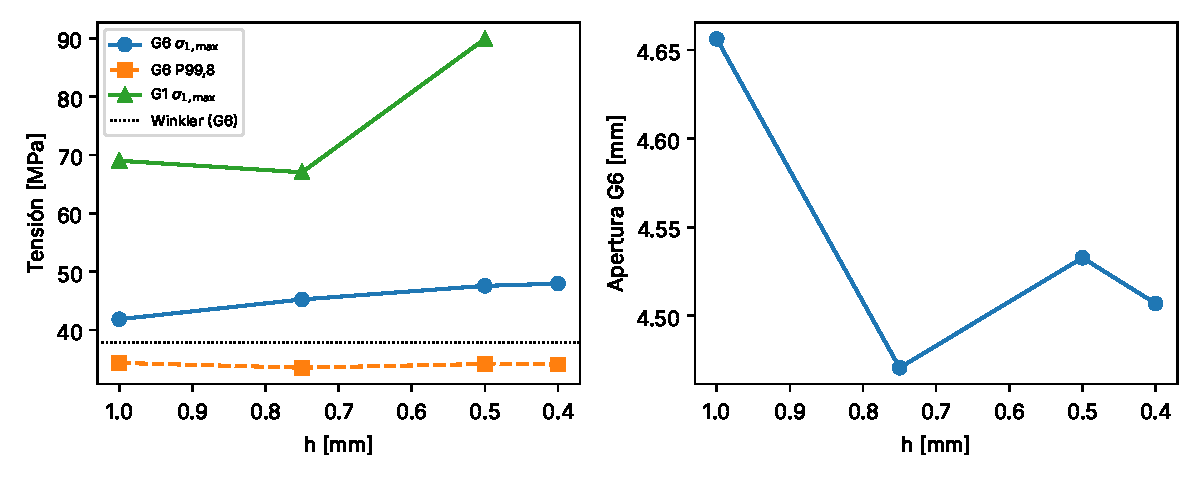
\includegraphics[width=0.9\linewidth]{../figures/convergencia.pdf}
\caption{Convergencia de malla en el caso 3 (macizo) y comparación con la solución de Winkler.}
\end{figure}

\paragraph{Contraste con vigas curvas.} En la corona, $N=F$ y $M=F\,e$ con $e=y_t-\bar y_{carga}=50{,}25$~mm. Para la sección circular de G6 ($R=22{,}5$, $c=6$~mm), Winkler~\cite{shigley} da $r_n=c^2/(2(R-\sqrt{R^2-c^2}))=22{,}093$~mm y $\sigma_i=\WinklerSi$~MPa ($K_i=\WinklerKi$ sobre la viga recta, $M/Z=\WinklerStraight$~MPa). El MEF macizo con $h=0{,}4$~mm da \FemMax~MPa como máximo y \FemPct~MPa en el percentil 99,8: los dos indicadores encierran la solución analítica (\FemMaxDev~\% y \FemPctDev~\%), con el pico en la fibra interior de la corona. La diferencia del máximo proviene de las esquinas entrantes de la superficie escalonada, de modo que las capacidades basadas en $\sigma_{1,\max}$ son conservadoras para las geometrías con arco, con el mismo sesgo en todos los materiales.

\section{Resultados mecánicos por geometría}
\begin{table}[htbp]
\centering\small
\caption{$\sigma_{1,\max}$ [MPa] en la cáscara para los tres casos de carga.}
\label{tab:casos}
\fitbox{
\begin{tabular}{lrrr}
\toprule
Geometría (5 paredes, 25 \%) & Caso 1: tiro, 200 N & Caso 2: 100 N/pata & Caso 3: 100 N/pata \\
\midrule
G1 $\cdot$ R6 (v5 actual) & 13{,}9 & 7{,}8 & 106{,}2 \\
G4 $\cdot$ R15 (v8) & 8{,}3 & 7{,}6 & 59{,}6 \\
G6 $\cdot$ arco R22,5 (v7) & 6{,}8 & 7{,}3 & 54{,}5 \\
\bottomrule
\end{tabular}}
\par\smallskip\parbox{0.95\linewidth}{\footnotesize En los casos 1 y 2 se excluye la zona empotrada ($y\le-22{,}5$ mm).}
\end{table}

El caso 3 produce tensiones entre \CaseRatioMin{} y \CaseRatioMax{} veces mayores que los casos 1 y 2 para la misma fuerza por pata: la fuerza actúa a unos 50~mm del tramo superior y genera $M\approx5000$~N\,mm en la corona. Es el caso de diseño y coincide con la falla observada.

\begin{table}[htbp]
\centering\small
\caption{Exploración geométrica, caso 3, 5 paredes y 25 \%, 100 N por pata, $E=3500$ MPa (tensiones en MPa).}
\label{tab:geom}
\fitbox{
\begin{tabular}{lrrrrrr}
\toprule
Geometría & $\sigma_{1,\max}$ & P99,8 & $\sigma_{VM,\max}$ & Apertura [mm] & Vol. [cm$^3$] & Ventana [mm$^2$] \\
\midrule
G1 $\cdot$ R6 (v5 actual) & 106{,}2 & 48{,}8 & 80{,}5 & 6{,}95 & 16{,}6 & 792 \\
G2 $\cdot$ R9 & 70{,}7 & 50{,}9 & 60{,}9 & 6{,}70 & 16{,}3 & 790 \\
G3 $\cdot$ R12 & 64{,}7 & 46{,}4 & 53{,}7 & 6{,}36 & 16{,}0 & 784 \\
G4 $\cdot$ R15 (v8) & 59{,}6 & 44{,}2 & 50{,}5 & 6{,}07 & 15{,}8 & 775 \\
G5 $\cdot$ R18 & 57{,}1 & 41{,}8 & 47{,}7 & 5{,}76 & 15{,}5 & 761 \\
G6 $\cdot$ Arco R22,5 (v7) & 54{,}5 & 40{,}6 & 45{,}3 & 5{,}32 & 15{,}1 & 734 \\
G7 $\cdot$ R15 + 14 mm adentro & 48{,}8 & 33{,}5 & 39{,}9 & 3{,}68 & 17{,}2 & 706 \\
G8 $\cdot$ R15 + 16 mm adentro & 39{,}4 & 28{,}2 & 32{,}6 & 2{,}45 & 18{,}3 & 645 \\
G9 $\cdot$ Arco + 14 mm adentro & 40{,}3 & 30{,}8 & 34{,}5 & 3{,}25 & 16{,}3 & 672 \\
G10 $\cdot$ Arco + 16 mm adentro & 33{,}4 & 24{,}2 & 28{,}6 & 2{,}14 & 17{,}3 & 616 \\
\bottomrule
\end{tabular}}
\par\smallskip\parbox{0.95\linewidth}{\footnotesize Ventana: área libre en el plano medio, en la mitad $x\ge0$.}
\end{table}

\begin{figure}[htbp]\centering
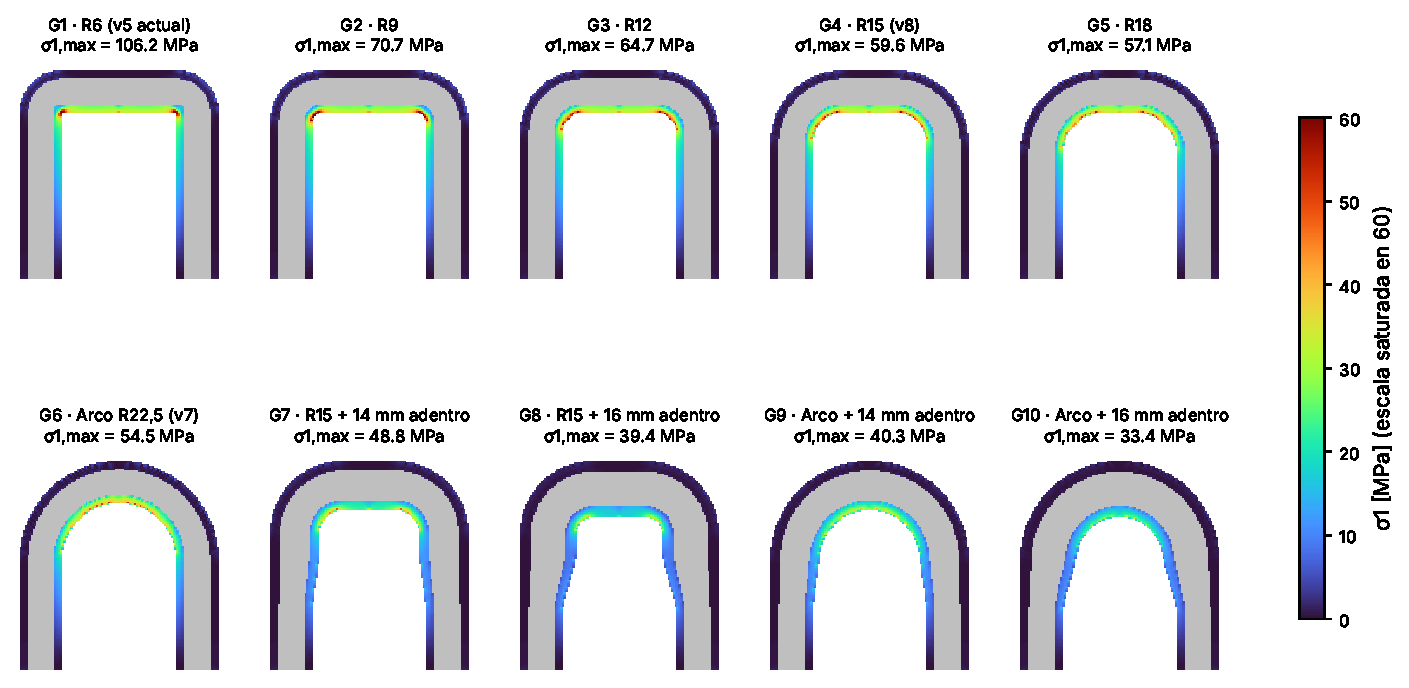
\includegraphics[width=\linewidth]{../figures/fig1_sigma1_geometrias.pdf}
\caption{Tensión principal máxima $\sone$ en el plano medio de las 10 geometrías, caso 3, 100~N por pata, 5 paredes y 25~\%. En gris, el núcleo de relleno.}
\end{figure}

El barrido de radio muestra rendimientos decrecientes: de R6 a R9 el pico baja un \RsixRnine~\% al eliminar la singularidad; de R9 al arco completo, otro \RnineArc~\%. Con $\varnothing$12 constante el límite lo pone el momento de la corona; para seguir bajando hay que aumentar su módulo resistente ($Z\propto A^2B$). \textbf{G10} (arco con la corona engrosada a 16~mm hacia adentro) es el óptimo de capacidad: \GtenVsGone{} veces la de la v5 y \GtenVsGsix{} veces la de la v7, con \VolGten{} frente a \VolGone~cm$^3$ de material, a cambio de \WinLossGten~\% menos de ventana. Si la ventana no se puede reducir, el óptimo restringido es G6 (v7), con \GsixVsGone{} veces la capacidad actual.

\begin{figure}[htbp]\centering
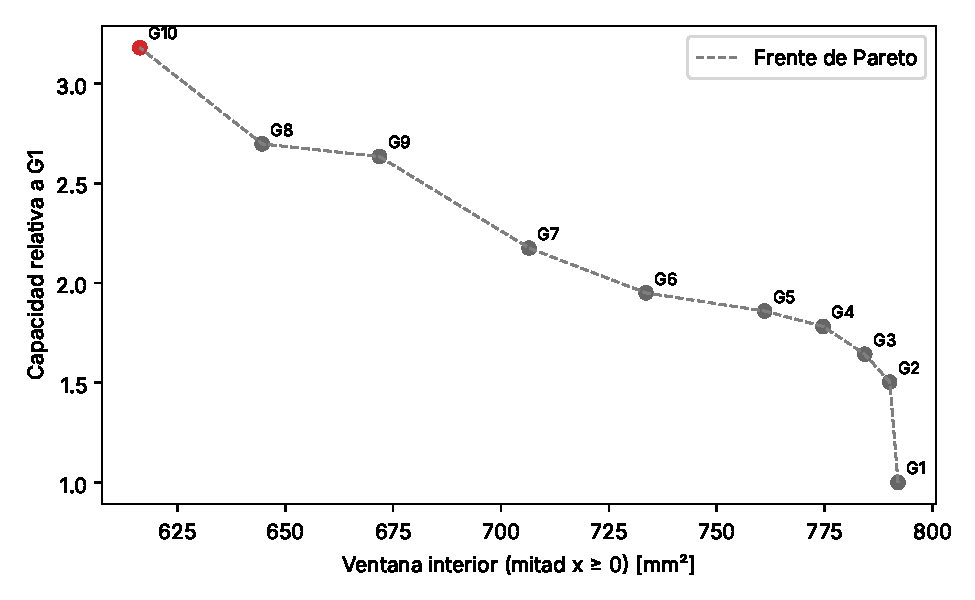
\includegraphics[width=0.7\linewidth]{../figures/pareto.pdf}
\caption{Capacidad relativa frente a la ventana interior.}
\end{figure}

\section{Comparación de materiales}
Con la v7 y 5 paredes, el PAHT-CF soporta \FuPAHT~N por pata, \PAHTvsPLA{} veces el PLA (\FuPLA~N), y el PC \FuPC~N (\PCvsPLA{} veces). El cambio de geometría y perfil (de v5 con 2 paredes a v7 con 5 paredes) multiplica la capacidad por \GainVfiveVseven{} en cualquier material; las dos decisiones se suman, y el PAHT-CF con la v7 resiste \GainTotal{} veces lo que resiste hoy el gancho de PLA.

\begin{figure}[htbp]\centering
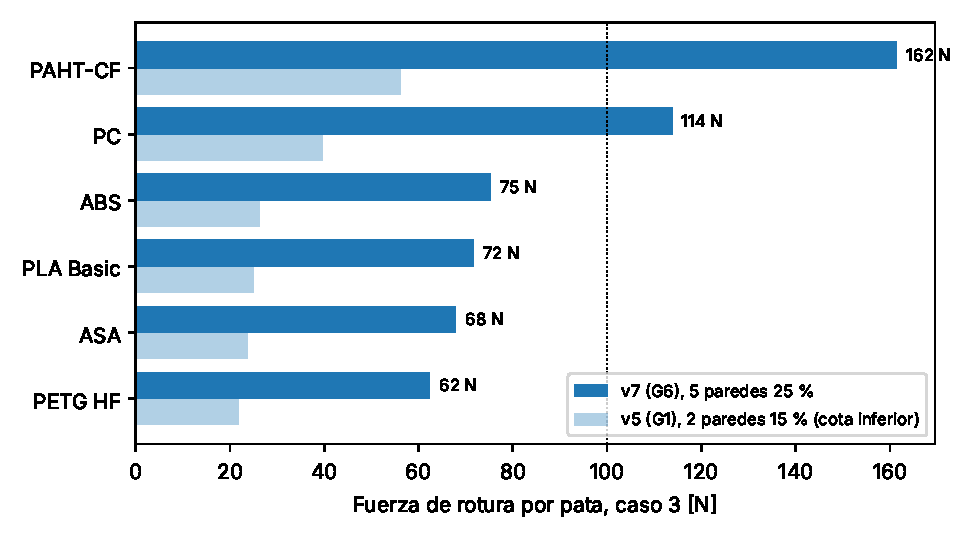
\includegraphics[width=0.75\linewidth]{../figures/capacidad_materiales.pdf}
\caption{Fuerza de rotura por pata según material y geometría.}
\end{figure}
\begin{figure}[htbp]\centering
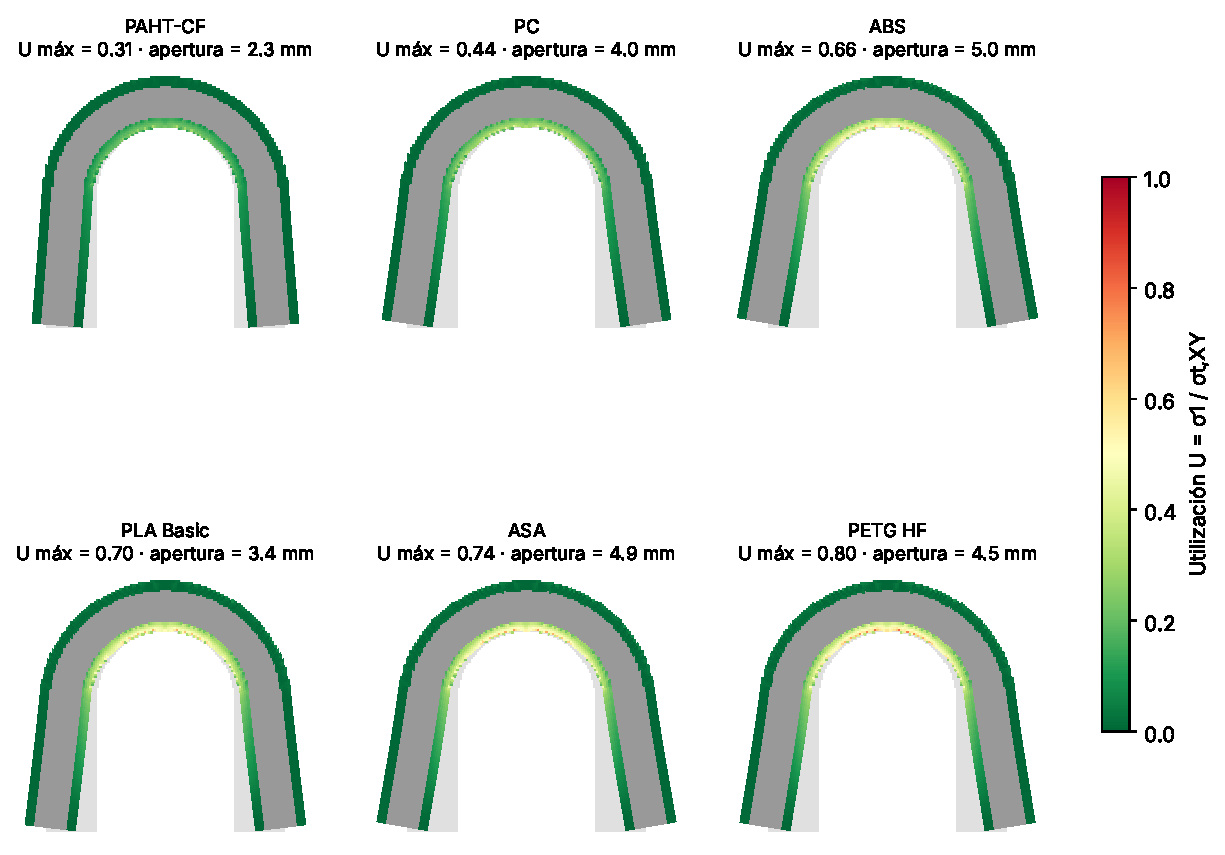
\includegraphics[width=0.95\linewidth]{../figures/fig2_utilizacion_v7.pdf}
\caption{Geometría v7 (G6) con 50~N por pata: utilización $U=\sone/\sigma_{t,XY}$ y deformada $\times3$ sobre la forma original. El campo de tensiones es el mismo en los seis paneles; cambian la utilización y la apertura.}
\end{figure}
\begin{figure}[htbp]\centering
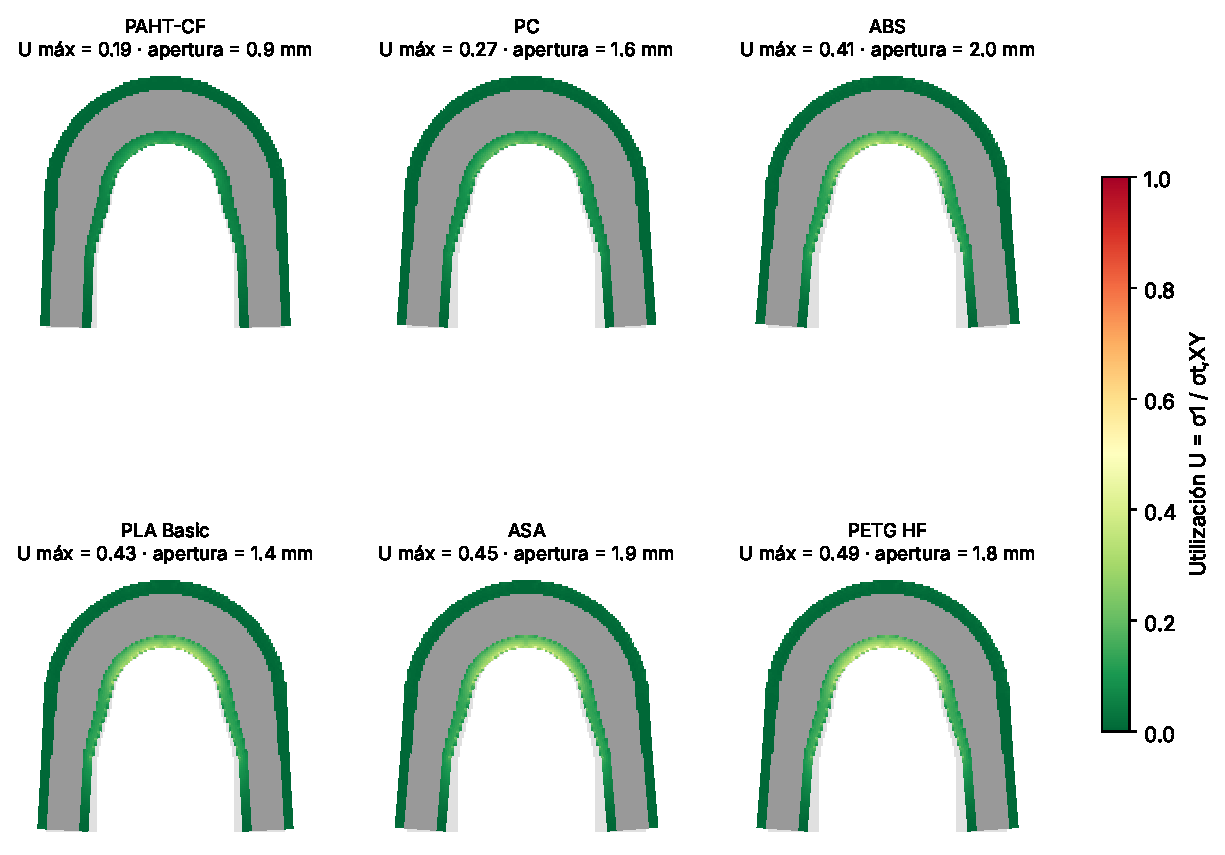
\includegraphics[width=0.95\linewidth]{../figures/fig3_utilizacion_G10.pdf}
\caption{Lo mismo para G10. La utilización máxima baja de \UPLAseven{} a \UPLAten{} en PLA y de \UPAHTseven{} a \UPAHTten{} en PAHT-CF.}
\end{figure}

\begin{table}[htbp]
\centering\small
\caption{Indicadores por material (5 paredes, 25 \%, caso 3).}
\label{tab:mat}
\fitbox{
\begin{tabular}{lrrrrrrr}
\toprule
Material & $F_u$ v7 [N] & $F_u$ v8 [N] & $F_{adm}$ sost. [N] & Apertura 50 N [mm] & $\varepsilon_b/\varepsilon_{pico}$ & Margen HDT [°C] & Impacto [kJ/m$^2$] \\
\midrule
PAHT-CF & 162 & 148 & 48 & 2{,}3 & 4{,}6 & 130 & 22{,}8 \\
PC & 114 & 104 & 34 & 4{,}0 & 1{,}3 & 77 & 7{,}5 \\
ABS & 75 & 69 & 23 & 5{,}0 & 9{,}7 & 44 & 21{,}5 \\
PLA Basic & 72 & 65 & 21 & 3{,}4 & 8{,}4 & 14 & 7{,}9 \\
ASA & 68 & 62 & 20 & 4{,}9 & 6{,}1 & 52 & 19{,}6 \\
PETG HF & 62 & 57 & 19 & 4{,}5 & 4{,}6 & 22 & 6{,}2 \\
\bottomrule
\end{tabular}}
\par\smallskip\parbox{0.95\linewidth}{\footnotesize $F_u = 100\,\mathrm{N}\cdot\sigma_{t,XY}/\sigma_{1,\max}$; sostenida con $\eta=0{,}3$; apertura escalada con el módulo de flexión; margen HDT con 40 °C de servicio.}
\end{table}


\begin{table}[htbp]\centering\small
\caption{Matriz de decisión.}
\begin{tabular}{llll}\toprule
Criterio & Mejor & Aceptable & Desfavorable\\\midrule
Capacidad a corto plazo & PAHT-CF, PC & ABS, PLA, ASA & PETG\\
Carga sostenida y fluencia & PC, PAHT-CF & ABS & PLA, ASA, PETG\\
Temperatura (HDT) & PAHT-CF, PC & ASA, ABS & PETG, PLA\\
Tenacidad al impacto & PAHT-CF, ABS, ASA & — & PLA, PC, PETG\\
Tolerancia a entallas & ABS, PLA, ASA & PAHT-CF, PETG & PC\\
Rigidez & PAHT-CF & PLA, PC & PETG, ASA, ABS\\
Facilidad de impresión & PLA, PETG & ASA, ABS & PC, PAHT-CF\\\bottomrule
\end{tabular}\end{table}


\section{Análisis no lineal: ¿con qué carga el gancho se estira?}\label{sec:nl}
En servicio, el problema habitual no es una rotura limpia sino que el gancho \emph{de repente se estira}: se abre y queda abierto. Eso es fluencia plástica en la corona (o en la esquina de la v5), que el análisis elástico no puede describir. Para cuantificarlo se resolvió el caso~3 con plasticidad y grandes desplazamientos.

\paragraph{Formulación.} Lagrangiana total con deformación de Green--Lagrange $\mathbf E=\frac12(\mathbf F^T\mathbf F-\mathbf I)$ y segundo tensor de Piola--Kirchhoff $\mathbf S$; plasticidad J2 (von Mises) con endurecimiento isótropo lineal, retorno radial y tangente consistente; hexaedro de 8 nodos con integración $2\times2\times2$ y el método $\bar{\mathbf E}$ (parte volumétrica media por elemento, análogo al B-bar) para evitar el bloqueo volumétrico del flujo plástico. Se usa un cuarto de modelo ($x\ge0$, $z\ge0$, condiciones de simetría) con $h=1$~mm. La carga es la misma fuerza uniforme del caso 3 sobre la cara exterior de la punta, con magnitud incógnita y control por desplazamiento de la apertura (sistema orlado), de modo que la curva se puede seguir incluso pasado un máximo.

\paragraph{Material.} Cáscara con $E=E_{t,XY}$, $\sigma_y=\sigma_{t,XY}$ y $H=0{,}01E$; el núcleo con $E$ y $\sigma_y$ escalados por $k$. Se definen tres cargas: la \textbf{1.ª fluencia} (primer punto de la cáscara que plastifica), la \textbf{carga de estiramiento} $F_{1\,mm}$ (la fuerza con la que, al descargar, queda 1~mm de apertura permanente; método del offset sobre la curva) y la \textbf{rotura estimada} (cuando la deformación plástica equivalente en la cáscara alcanza $\varepsilon_b-\sigma_t/E_t$ de la ficha).

\paragraph{Control del modelo.} Refinar a $h=0{,}75$~mm cambia $F_{1\,mm}$ un \NLmeshOff~\% y la rotura un \NLmeshRup~\% (PLA, v7). Quitar el endurecimiento ($H=0$) cambia $F_{1\,mm}$ un \NLhardOff~\% y la rotura un \NLhardRup~\%. Las cargas de la v5 con canto vivo sí dependen de la malla (singularidad) y deben leerse como indicativas.

\begin{figure}[htbp]\centering
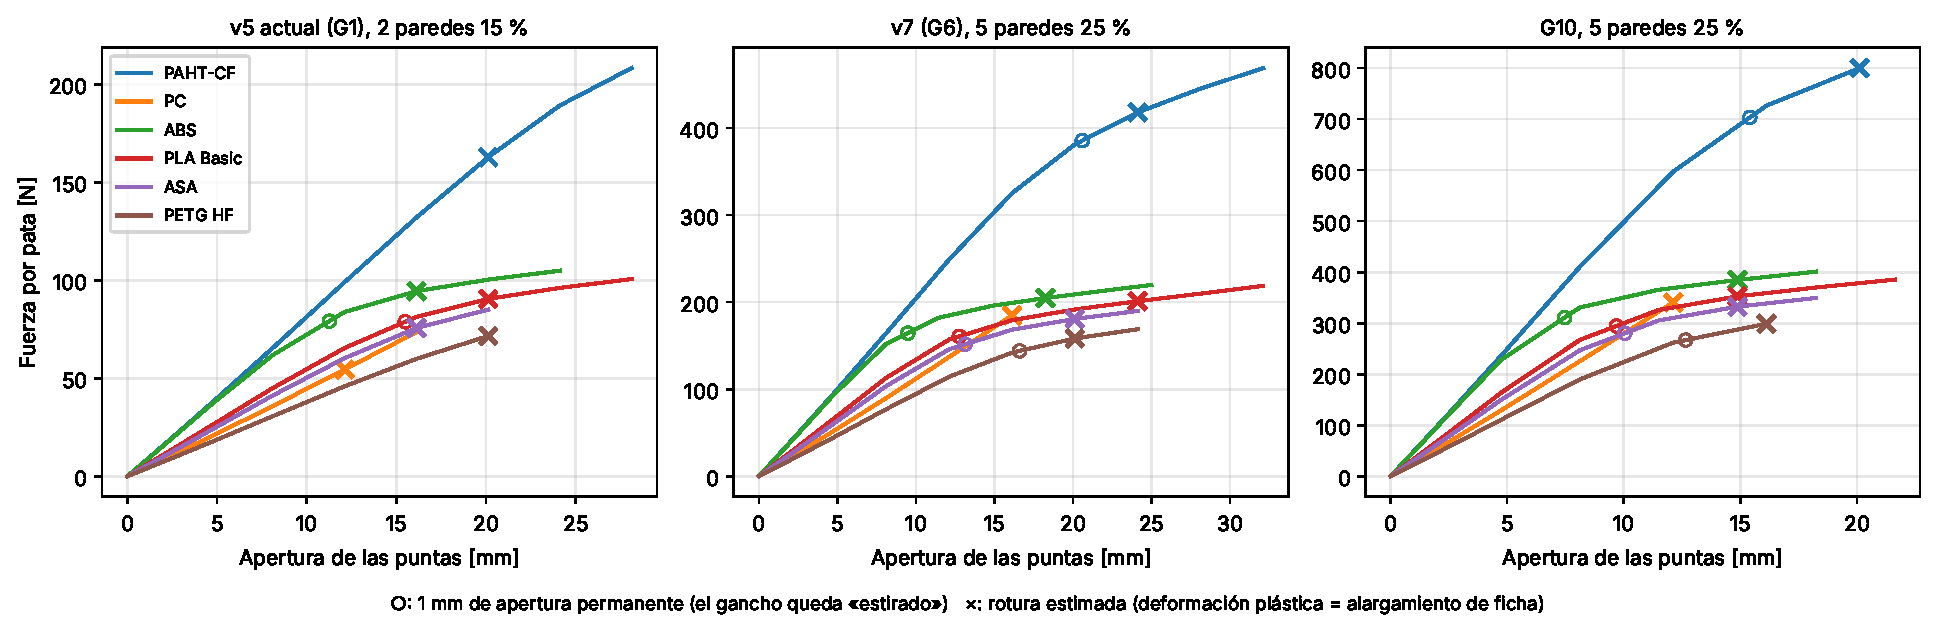
\includegraphics[width=\linewidth]{../figures/nl_fuerza_apertura.pdf}
\caption{Curvas fuerza--apertura no lineales, caso 3. Círculo: 1~mm de apertura permanente. Cruz: rotura estimada.}
\end{figure}
\begin{table}[htbp]
\centering\small
\caption{Análisis no lineal (plasticidad J2 + grandes desplazamientos), caso 3. Fuerzas por pata en N.}
\label{tab:nl}
\fitbox{
\begin{tabular}{llrrrrr}
\toprule
Geometría & Material & $F_u$ lineal & 1.ª fluencia & $F_{1\,mm}$ permanente & $F$ rotura & Apertura en rotura [mm] \\
\midrule
G1 (2p) & PAHT-CF & 56 & 66 & — & 163 & 20{,}1 \\
G1 (2p) & PC & 40 & 54 & — & 54 & 12{,}1 \\
G1 (2p) & ABS & 26 & 37 & 79 & 94 & 16{,}1 \\
G1 (2p) & PLA Basic & 25 & 26 & 79 & 90 & 20{,}1 \\
G1 (2p) & ASA & 24 & 24 & — & 76 & 16{,}1 \\
G1 (2p) & PETG HF & 22 & 31 & — & 72 & 20{,}1 \\
G6 (5p) & PAHT-CF & 162 & 249 & 386 & 418 & 24{,}1 \\
G6 (5p) & PC & 114 & 137 & — & 185 & 16{,}1 \\
G6 (5p) & ABS & 75 & 93 & 164 & 205 & 18{,}2 \\
G6 (5p) & PLA Basic & 72 & 113 & 161 & 201 & 24{,}1 \\
G6 (5p) & ASA & 68 & 104 & 152 & 181 & 20{,}1 \\
G6 (5p) & PETG HF & 62 & 77 & 144 & 158 & 20{,}1 \\
G10 (5p) & PAHT-CF & 263 & 411 & 703 & 800 & 20{,}1 \\
G10 (5p) & PC & 186 & 226 & — & 341 & 12{,}1 \\
G10 (5p) & ABS & 123 & 228 & 311 & 385 & 14{,}9 \\
G10 (5p) & PLA Basic & 117 & 164 & 295 & 352 & 14{,}9 \\
G10 (5p) & ASA & 111 & 150 & 280 & 332 & 14{,}9 \\
G10 (5p) & PETG HF & 102 & 190 & 267 & 299 & 16{,}1 \\
\bottomrule
\end{tabular}}
\par\smallskip\parbox{0.95\linewidth}{\footnotesize $F_u$ lineal: criterio de Rankine del análisis elástico (sección 10). 1.ª fluencia: primer punto de Gauss de la cáscara que plastifica (von Mises). $F_{1\,mm}$: fuerza con la que, al descargar, queda 1 mm de apertura permanente. —: el material rompe antes de llegar a ese punto.}
\end{table}


\paragraph{Resultados.} (i) En los materiales dúctiles la curva tiene un codo marcado: tras la 1.ª fluencia se forma una rótula plástica en la corona y la apertura crece mucho con poco aumento de carga. Ese es el «estiramiento repentino» observado. (ii) La carga de estiramiento vale entre \NLratioMin{} y \NLratioMax{} veces la capacidad elástica de la sección~10: el criterio lineal es conservador para la rotura, pero marca bien dónde empieza el daño permanente. (iii) En la v7, el PLA se estira con unos \NLoffPLAsix~N por pata y el PETG con \NLoffPETGsix~N; el PAHT-CF necesita \NLoffPAHTsix~N. (iv) El PC no se estira: con su reserva de ductilidad de \DuctPC{} rompe (\NLrupPCsix~N en la v7) antes de acumular 1~mm de deformación permanente. Es frágil, sin aviso. (v) En G10, el PLA se estira con \NLoffPLAten~N y el PAHT-CF con \NLoffPAHTten~N por pata.

\paragraph{Lectura práctica.} Si el gancho actual «se estira de repente», la causa es plastificación de la esquina con cargas de pico, no fluencia lenta. Las dos palancas son las mismas que en el análisis elástico (geometría con arco y corona engrosada, y un material más resistente), pero aquí se ve además el modo de falla: PLA, ABS, ASA, PETG y PAHT-CF avisan deformándose; el PC no.

\section{Fluencia lenta bajo carga sostenida}\label{sec:creep}
Con viscoelasticidad lineal y $\nu$ constante, el principio de correspondencia aplicado al teorema de la sección~4.2 da un resultado útil: bajo carga constante \textbf{la tensión no cambia con el tiempo} y la apertura crece con la flexibilidad de fluencia,
\begin{equation}
\Delta(t)=\Delta_{ref}\,\frac{E_{ref}}{E_{f,XY}}\,\frac{F}{F_{ref}}\,\bigl[1+\varphi(t)\bigr],\qquad \varphi(t)=(t/\tau)^n\ \text{(Findley)}.
\end{equation}
Las fichas no dan $\varphi(t)$ y la literatura disponible~\cite{dogan,hausler} solo ordena los materiales. Por eso se usaron \emph{escenarios} de Findley ($n=0{,}2$) que respetan ese orden, con $\varphi(1000\,\text{h})$ entre 0,3 (PC) y 1,0 (PLA). No son datos de ensayo: sirven para ver órdenes de magnitud y se deben calibrar con un ensayo de peso colgado sobre piezas impresas (\texttt{scripts/ajuste\_fluencia.py} ajusta $\tau$ y $n$ a las mediciones).

\begin{figure}[htbp]\centering
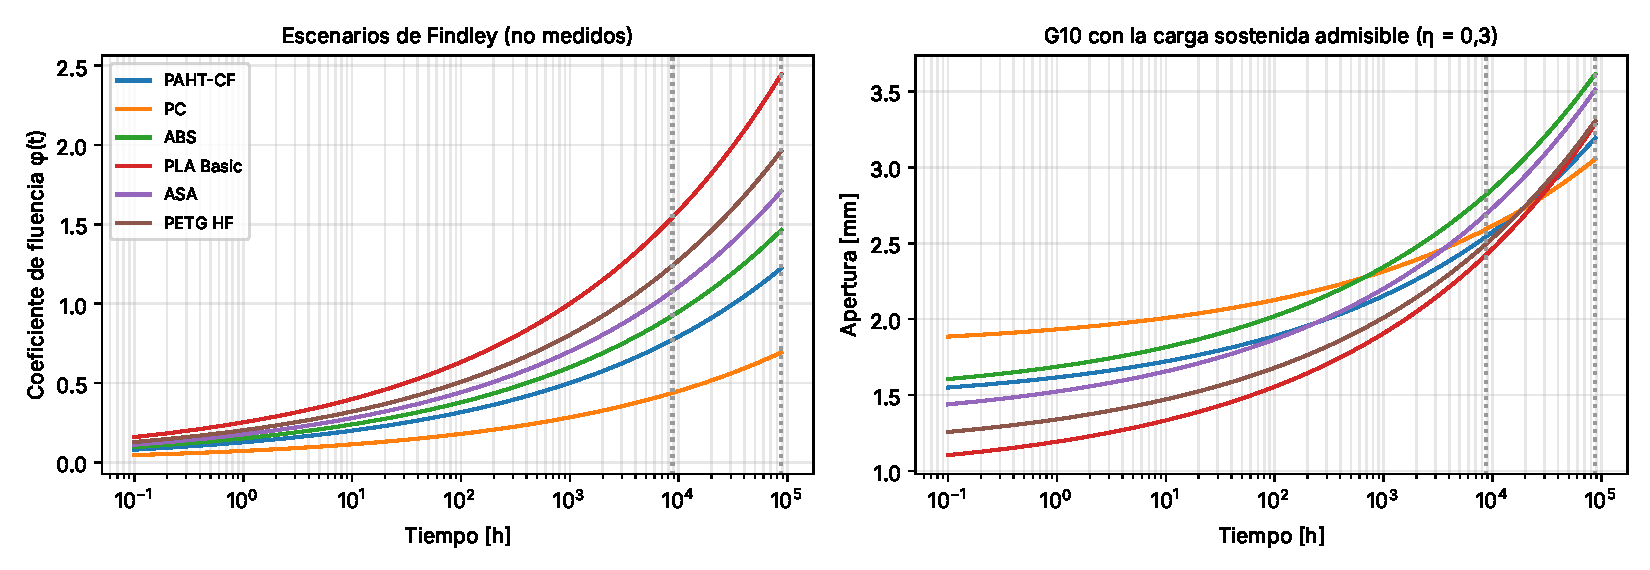
\includegraphics[width=0.95\linewidth]{../figures/fluencia.pdf}
\caption{Escenarios de fluencia y apertura en el tiempo de G10 con la carga sostenida admisible ($\eta=0{,}3$).}
\end{figure}
\begin{table}[htbp]
\centering\small
\caption{Apertura bajo la carga sostenida admisible ($\eta=0{,}3$), por fluencia lenta a 23 °C.}
\label{tab:creep}
\fitbox{
\begin{tabular}{llrrrrr}
\toprule
Geom. & Material & $F_{sost}$ [N] & $\Delta_0$ [mm] & $\varphi$(1000 h) & $\Delta$ 1 año [mm] & $\Delta$ 10 años [mm] \\
\midrule
G6 & PAHT-CF & 48 & 2{,}19 & 0{,}50 & 3{,}88 & 4{,}87 \\
G10 & PAHT-CF & 79 & 1{,}44 & 0{,}50 & 2{,}54 & 3{,}19 \\
G6 & PC & 34 & 2{,}75 & 0{,}28 & 3{,}96 & 4{,}66 \\
G10 & PC & 56 & 1{,}80 & 0{,}28 & 2{,}59 & 3{,}05 \\
G6 & ABS & 23 & 2{,}24 & 0{,}60 & 4{,}31 & 5{,}52 \\
G10 & ABS & 37 & 1{,}47 & 0{,}60 & 2{,}82 & 3{,}61 \\
G6 & PLA Basic & 21 & 1{,}46 & 1{,}00 & 3{,}70 & 5{,}02 \\
G10 & PLA Basic & 35 & 0{,}95 & 1{,}00 & 2{,}42 & 3{,}29 \\
G6 & ASA & 20 & 1{,}98 & 0{,}70 & 4{,}11 & 5{,}36 \\
G10 & ASA & 33 & 1{,}30 & 0{,}70 & 2{,}69 & 3{,}51 \\
G6 & PETG HF & 19 & 1{,}70 & 0{,}80 & 3{,}81 & 5{,}04 \\
G10 & PETG HF & 31 & 1{,}11 & 0{,}80 & 2{,}50 & 3{,}30 \\
\bottomrule
\end{tabular}}
\par\smallskip\parbox{0.95\linewidth}{\footnotesize Los coeficientes de fluencia son escenarios de Findley que respetan el orden cualitativo de [14, 15], no datos de ensayo. Calibrar con \texttt{scripts/ajuste\_fluencia.py}.}
\end{table}


Con la carga sostenida admisible ($\eta=0{,}3$; \CrPAHTF~N por pata en PAHT-CF y \CrPLAF~N en PLA con G10), la apertura pasaría de \CrPLAzero{} a \CrPLAten~mm en 10 años en PLA, de \CrPCzero{} a \CrPCten~mm en PC y de \CrPAHTzero{} a \CrPAHTten~mm en PAHT-CF. Con $\eta=0{,}3$ la tensión queda lejos de la fluencia plástica (sección~\ref{sec:nl}), así que el riesgo con carga permanente es una apertura que crece lentamente, no un estiramiento brusco. La temperatura domina: a 40--60~°C el PLA rompe por fluencia en horas~\cite{dogan}, lo que refuerza la recomendación de PAHT-CF o PC si el gancho trabaja caliente.

\section{Discusión y limitaciones}
\paragraph{Anisotropía.} El teorema de escalado supone isotropía. Los materiales reales tienen $E_Z/E_{XY}$ entre 0,56 (PAHT-CF) y 0,87 (ASA). En el caso 3 el gancho es globalmente isostático: los esfuerzos internos quedan fijados por el equilibrio y la anisotropía solo redistribuye la tensión dentro de la sección. Como la pieza se imprime acostada, la flexión en el plano de la U produce tensiones a lo largo de las capas y la dirección débil solo recibe cortante interlaminar, nulo en las fibras extremas.
\paragraph{Pieza frente a probeta.} Las resistencias provienen de probetas macizas, recocidas y secas; una pieza real tiene defectos, por lo que se recomienda $FS\ge2$.
\paragraph{Singularidad de la v5.} Su capacidad depende de la plasticidad local y queda entre las cotas informadas.
\paragraph{No linealidades.} El análisis lineal es levemente conservador en lo geométrico; en materiales dúctiles la plastificación local redistribuye tensiones, lo que casi no ocurre en el PC (reserva \DuctPC).
\paragraph{Fluencia y humedad.} $\eta=0{,}3$ es una hipótesis común; no hay datos de fluencia para este grado de PAHT-CF y su absorción de agua reduce sus propiedades.
\paragraph{No modelado.} Contacto con el tope, tensiones residuales, fatiga, UV y ataque químico. Se recomienda validar con ensayos de rotura de al menos 3 piezas por material.

\section{Conclusiones y material recomendado}
\textbf{Material recomendado: PAHT-CF}; si la impresora no tiene boquilla endurecida o no se puede secar el filamento, la alternativa es el PC.
\begin{enumerate}
\item La falla observada es la del caso 3. El gancho actual (G1, PLA, 2 paredes) empieza a romperse con \FuFivePLAlo--\FuFivePLAhi~N por pata.
\item Con cargas impuestas, la tensión no depende del material: la capacidad es proporcional a $\sigma_{t,XY}$ y la apertura inversamente proporcional al módulo de flexión.
\item En la v7 con 5 paredes, el PAHT-CF resiste \FuPAHT~N por pata, el PC \FuPC~N y el PLA \FuPLA~N. Con 50~N por pata la utilización máxima es \UPAHTseven{} en PAHT-CF, \UPCseven{} en PC, \UPLAseven{} en PLA y \UPETGseven{} en PETG.
\item El PETG no conviene para este gancho; el ASA conviene si trabaja al aire libre.
\item La geometría pesa tanto como el material: G10 da \GtenVsGone{} veces la capacidad de la v5.
\item El «estiramiento repentino» es plastificación de la corona o la esquina. En la v7 el PLA queda con 1~mm de apertura permanente a unos \NLoffPLAsix~N por pata; con G10 en PAHT-CF hacen falta unos \NLoffPAHTten~N. El PC no se estira: rompe sin aviso.
\item Con la carga sostenida admisible la tensión no cambia en el tiempo y la apertura crece por fluencia (de \CrPLAzero{} a \CrPLAten~mm en 10 años en PLA, según los escenarios); conviene calibrarla con un ensayo de carga colgada.
\item \textbf{Combinación óptima: G10 en PAHT-CF con 5 paredes y 25~\% gyroid}, con unos \FuTenPAHT~N por pata a la rotura, \FuTenPAHTadm~N admisibles con $FS=2$ y unos \FuTenPAHTsost~N de carga permanente con $\eta=0{,}3$. En PC, la misma geometría llega a \FuTenPC~N.
\end{enumerate}

\appendix
\section{Modelos imprimibles}
La carpeta \texttt{modelos\_stl/} contiene un STL cerrado por geometría (G1--G10), generado por \emph{marching cubes} sobre la misma función implícita $\varphi$ del MEF (\texttt{scripts/export\_stl.py}), en mm, con la U acostada en el plano de la cama como en el estudio. Para la recomendación final se imprime \texttt{gancho\_G10.stl} (o \texttt{gancho\_G6.stl} si se necesita la ventana completa) con 5 paredes y 25~\% gyroid.

\section{Código y reproducibilidad}\label{app:codigo}
Todo el cálculo de este informe lo produce el paquete \texttt{ganchofem} del repositorio:
\begin{lstlisting}
pip install -r requirements.txt
python scripts/run_all.py --jobs 3     # 63 simulaciones
python scripts/run_nonlinear.py --jobs 3  # analisis no lineal (20 corridas)
python scripts/postprocess.py          # tablas, figuras y cifras
python scripts/export_stl.py           # modelos imprimibles
cd report && latexmk -pdf informe.tex  # este PDF
pytest -q                              # pruebas automaticas
\end{lstlisting}
La comparación con las cifras del estudio original está en \texttt{results/comparacion.md}, y las diferencias de método en \texttt{docs/diferencias.md}. En resumen: con $h=0{,}5$~mm las mallas tienen los mismos elementos y grados de libertad que el estudio original, y todas las tensiones y aperturas del caso 3 quedan dentro de $+0{,}4$~\%.

\begin{thebibliography}{99}\small
\bibitem{zienkiewicz} O.~C. Zienkiewicz, R.~L. Taylor y J.~Z. Zhu, \emph{The Finite Element Method: Its Basis and Fundamentals}, 7.ª ed. Butterworth-Heinemann, 2013.
\bibitem{shigley} R.~G. Budynas y J.~K. Nisbett, \emph{Shigley's Mechanical Engineering Design}, 11.ª ed. McGraw-Hill, 2020, sec.~3-18.
\bibitem{sinclair} G.~B. Sinclair, ``Stress singularities in classical elasticity--I,'' \emph{Applied Mechanics Reviews}, 57(4):251--298, 2004.
\bibitem{keyak1990} J.~H. Keyak et al., ``Automated three-dimensional finite element modelling of bone: a new method,'' \emph{J. Biomed. Eng.}, 12(5):389--397, 1990.
\bibitem{keyak1992} J.~H. Keyak y H.~B. Skinner, ``Three-dimensional finite element modelling of bone: effects of element size,'' \emph{J. Biomed. Eng.}, 14(6):483--489, 1992.
\bibitem{farah} S. Farah, D.~G. Anderson y R. Langer, ``Physical and mechanical properties of PLA...,'' \emph{Adv. Drug Deliv. Rev.}, 107:367--392, 2016.
\bibitem{chacon} J.~M. Chacón et al., ``Additive manufacturing of PLA structures using FDM...,'' \emph{Materials \& Design}, 124:143--157, 2017.
\bibitem{ahn} S.-H. Ahn et al., ``Anisotropic material properties of fused deposition modeling ABS,'' \emph{Rapid Prototyping J.}, 8(4):248--257, 2002.
\bibitem{fernandez} M. Fernandez-Vicente et al., ``Effect of infill parameters on tensile mechanical behavior in desktop 3D printing,'' \emph{3D Print. Addit. Manuf.}, 3(3), 2016.
\bibitem{waseem} M. Waseem et al., ``Multi-response optimization of tensile creep behavior of PLA 3D printed parts...,'' \emph{Polymers}, 12(12):2962, 2020.
\bibitem{gibson} L.~J. Gibson y M.~F. Ashby, \emph{Cellular Solids}, 2.ª ed. Cambridge University Press, 1997.
\bibitem{dogan} O. Dogan, ``Short-term creep behaviour of different polymers used in additive manufacturing...,'' \emph{Stroj. vestn. -- J. Mech. Eng.}, 68(7--8):451--460, 2022.
\bibitem{hausler} P. Hausler et al., ``Evaluation of the creep strength of samples produced by fused deposition modeling,'' \emph{Open Engineering}, 14(1):20240084, 2024.
\bibitem{scipy} P. Virtanen et al., ``SciPy 1.0,'' \emph{Nature Methods}, 17:261--272, 2020.
\bibitem{numpy} C.~R. Harris et al., ``Array programming with NumPy,'' \emph{Nature}, 585:357--362, 2020.
\bibitem{bl-pla} Bambu Lab, \emph{PLA Basic -- Technical Data Sheet}, V2.0.
\bibitem{bl-petg} Bambu Lab, \emph{PETG HF -- Technical Data Sheet}, V1.0.
\bibitem{bl-asa} Bambu Lab, \emph{ASA -- Technical Data Sheet}, V3.0.
\bibitem{bl-abs} Bambu Lab, \emph{ABS -- Technical Data Sheet}, V2.0.
\bibitem{bl-pc} Bambu Lab, \emph{PC -- Technical Data Sheet}, V2.0.
\bibitem{bl-paht} Bambu Lab, \emph{PAHT-CF -- Technical Data Sheet}, V2.0.
\end{thebibliography}
\end{document}
